\documentclass[a4paper,11pt]{article}
\usepackage[margin=18mm]{geometry}
\usepackage{tikz}
\pagestyle{empty}

\begin{document}
\begin{center}
{\Large Public Drawing (D1)}\\
{\small coordRef=public-grid-2400x3600, origin=top-left, unit=grid}
\end{center}

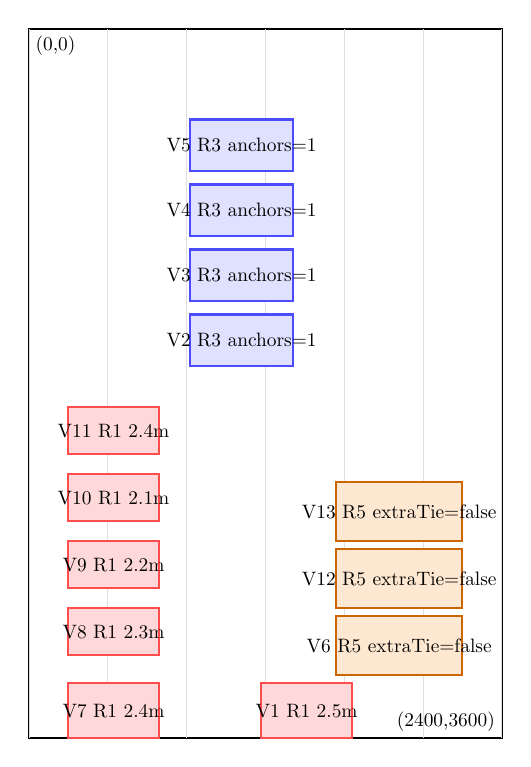
\begin{tikzpicture}[x=0.0025cm,y=-0.0025cm]
  \draw[black, thick] (0,0) rectangle (2400,3600);
  \draw[step=400,gray!25,very thin] (0,0) grid (2400,3600);
  \node[anchor=north west,scale=0.7] at (0,0) {(0,0)};
  \node[anchor=south east,scale=0.7] at (2400,3600) {(2400,3600)};

  % R1 (spacing): red
  \draw[draw=red!70,fill=red!15,thick] (1180,3320) rectangle (1640,3600);
  \node[scale=0.7] at (1410,3460) {V1 R1 2.5m};

  \draw[draw=red!70,fill=red!15,thick] (200,3320) rectangle (660,3600);
  \node[scale=0.7] at (430,3460) {V7 R1 2.4m};

  \draw[draw=red!70,fill=red!15,thick] (200,2940) rectangle (660,3180);
  \node[scale=0.7] at (430,3060) {V8 R1 2.3m};

  \draw[draw=red!70,fill=red!15,thick] (200,2600) rectangle (660,2840);
  \node[scale=0.7] at (430,2720) {V9 R1 2.2m};

  \draw[draw=red!70,fill=red!15,thick] (200,2260) rectangle (660,2500);
  \node[scale=0.7] at (430,2380) {V10 R1 2.1m};

  \draw[draw=red!70,fill=red!15,thick] (200,1920) rectangle (660,2160);
  \node[scale=0.7] at (430,2040) {V11 R1 2.4m};

  % R3 (anchor count): blue
  \draw[draw=blue!70,fill=blue!12,thick] (820,1450) rectangle (1340,1710);
  \node[scale=0.7] at (1080,1580) {V2 R3 anchors=1};

  \draw[draw=blue!70,fill=blue!12,thick] (820,1120) rectangle (1340,1380);
  \node[scale=0.7] at (1080,1250) {V3 R3 anchors=1};

  \draw[draw=blue!70,fill=blue!12,thick] (820,790) rectangle (1340,1050);
  \node[scale=0.7] at (1080,920) {V4 R3 anchors=1};

  \draw[draw=blue!70,fill=blue!12,thick] (820,460) rectangle (1340,720);
  \node[scale=0.7] at (1080,590) {V5 R3 anchors=1};

  % R5 (extra tie): orange
  \draw[draw=orange!80!black,fill=orange!18,thick] (1560,2980) rectangle (2200,3280);
  \node[scale=0.7] at (1880,3130) {V6 R5 extraTie=false};

  \draw[draw=orange!80!black,fill=orange!18,thick] (1560,2640) rectangle (2200,2940);
  \node[scale=0.7] at (1880,2790) {V12 R5 extraTie=false};

  \draw[draw=orange!80!black,fill=orange!18,thick] (1560,2300) rectangle (2200,2600);
  \node[scale=0.7] at (1880,2450) {V13 R5 extraTie=false};
\end{tikzpicture}

\vspace{4mm}
\noindent
\textbf{Legend.} Red=R1 (spacing), Blue=R3 (anchor count), Orange=R5 (extra tie).\\
Locators in the public reproduction dataset reference these rectangles via \texttt{bbox(x,y,w,h)} under \texttt{coordRef=public-grid-2400x3600}.

\end{document}
